\begin{tikzpicture}
\node [mybox] (box){%
    \begin{minipage}{0.3\textwidth}
    \begin{tabular}{p{0.3\textwidth} p{0.61\textwidth}}
      \vspace{-5pt}\hspace{-0.8cm} 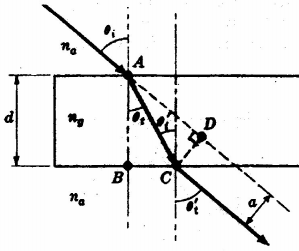
\includegraphics[scale=0.3]{images/ex_8.png} &
      \vspace{-8pt}
      \txt{
        \hspace{-0.5cm}
        \textbf{\textit{a) Angle du rayon lumineux sortant de la plaque?}}
        \par\hspace{-0.5cm}
        Interface 1:
        \par\hspace{-0.5cm}
        $nSolve(1.0sin30^\circ = 1.5sin\theta_{t1}, \theta_{t1})=19.47^\circ$
        \par\hspace{-0.5cm}
        Interface 2:
        \par\hspace{-0.5cm}
        $nSolve(1.5sin\theta_{t1} = 1.0sin\theta_{t2}, \theta_{t2})=30^\circ$
        \par\hspace{-0.5cm}
        $\alpha = 30 - 19.47$
        \par\hspace{-0.5cm}
        \textbf{\textit{b) Déplacement latéral "a" du rayon lumineux?}}
        \par\hspace{-0.5cm}
        $b\cdot cos \theta_{t1} \Rightarrow b=5.3cm$
        \par\hspace{-0.5cm}
        $5.3 sin (\theta_{t2}-\theta_{t1})=a=0.97cm$
      }
    \end{tabular}
    \end{minipage}
};
% \node[fancytitle, right=10pt] at (box.north west) {Exercice optique physique};
\end{tikzpicture}